\documentclass[a4paper,12pt]{report}
\usepackage{float}
\usepackage{setspace}
\usepackage[utf8]{inputenc}
\usepackage[T1]{fontenc}
\usepackage[english]{babel}
\usepackage{xcolor,graphicx, tikz}
\usepackage[top=0.3in,bottom=0in,right=1in,left=1in]{geometry}
\usepackage{background}
\usepackage{hyperref, url, float}
\usepackage{titlesec}
\usepackage{listings}
\usepackage{color}
\usepackage{minted}
\usepackage{tcolorbox}
\usepackage{xcolor}
\usepackage{xurl}

\definecolor{codegreen}{rgb}{0,0.6,0}
\definecolor{codegray}{rgb}{0.5,0.5,0.5}
\definecolor{codepurple}{rgb}{0.58,0,0.82}
\definecolor{backcolour}{rgb}{1,1,1}

\hypersetup{
    colorlinks=true,
    linkcolor=black,
    urlcolor=blue,
    pdfborder={0 0 0}, % Set border color to black
}
\usepackage{fix-cm}
\usepackage[bf]{caption}
\usepackage{subcaption}
\usepackage{amssymb}
\usepackage[fleqn]{amsmath,mathtools}
\usepackage{fancyhdr}
\usepackage[Lenny]{fncychap}
\usepackage{hyperref}
\ChTitleVar{\Huge\bfseries}
\ChNameVar{\large\bfseries}
\ChNumVar{\fontsize{60}{62}\bfseries}

%\setcounter{tocdepth}{4}

\setlength{\parskip}{0.2cm} % Set vertical space between paragraphs to 0.2cm

\titleformat{\section}{\normalfont\Large\bfseries}{\thesection}{1em}{}
\titlespacing*{\section}{0pt}{3pt}{2pt}
% Define background image
\usepackage{array}
\newcolumntype{P}[1]{>{\centering\arraybackslash}p{#1}}


\begin{document}
\begin{titlepage}
    \backgroundsetup{
    contents={\includegraphics[width=1.5cm,height=\paperheight]{Pics/rightPadUMI.jpeg}}, 
    angle=0,
    position=current page.east,
    vshift=0pt,
    hshift=0pt,
    opacity=1,
    scale=1
    }
    \begin{center}
        
        \begin{minipage}{13cm}
        	\begin{center}
        		\includegraphics[width=8.5cm,height=2.5cm]{Pics/LOGO_FS2_rapport.jpg}
        	\end{center}
        \end{minipage}\hfill
        
        
        %\includegraphics[width=0.6\textwidth]{logo-isae-supaero}\\[1cm]
        \textsc{\Large }\\[1cm]
        {{\fontsize{18pt}{18pt}\selectfont\textbf{Department of IT}}}\\[0.6cm]
        {\large \textbf{ Licence Program :}}\\[0.6cm]
        {\large \textbf{Mathematical Sciences and Computer Science (SMI)}}\\[2cm]
        
        { {\fontsize{26pt}{26pt}\selectfont\textbf{End-of-studies project}}\\[1.5cm] }
        \begin{flushleft}
             {\large \bfseries On the topic:}
        \end{flushleft}
       
        % Title
        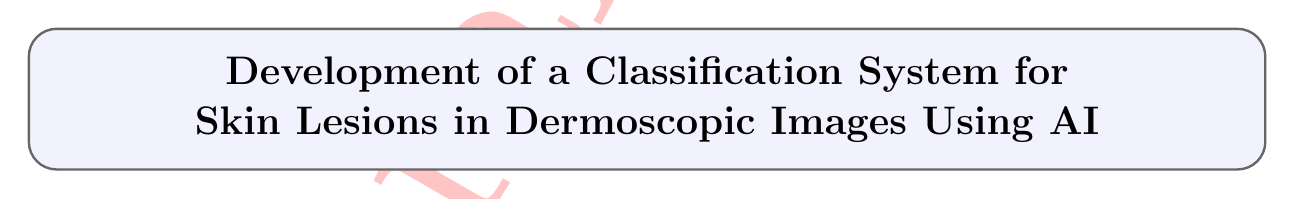
\begin{tikzpicture}
            \node[
                draw=black!60,
                line width=0.3mm,
                fill=blue!5,
                rounded corners=10pt,
                inner sep=10pt,
                align=center,
                text width=15cm,
                font=\Large\bfseries\color{black!70!black}
            ] 
            {Development of a Classification System for Skin Lesions in Dermoscopic Images Using AI};
        \end{tikzpicture}

        \noindent
        \begin{flushleft}
              \bf{Presented by :} \hspace{1.1cm} \textsc
            ~EL AMRAOUI \textbf{Khalil} \hspace{0.25cm} \&  \hspace{0.25cm} \textsc~TARIQ \textbf{Mohammed} 

        \end{flushleft}
        \begin{flushleft}
              \textbf{Supervised by :} \hspace{1cm} \textbf{Pr. \textsc{EL ANSARI } ~Mohamed} \hspace{2cm}
            \end{flushleft}

    \begin{flushleft}
         {\large \textit{Defended on Friday, 21st of June 2025, before the jury : }}\\[0.5cm]
    \end{flushleft}

%     \begin{tabular}{lll}
%         \bf \textbf{Pr. ~Abdelbaki \textsc{EL BELRHITI EL ALAOUI}}&  :&\bf \large Professeur à la FSM
%         \\[0.1cm]
%         \bf \textbf{Pr. ~Abdeslam \textsc{ELFERGOUGUI}}&  :&\bf \large Professeur à la FSM
%         \\[0.1cm]
%         \bf \textbf{Pr. ~El Mehdi \textsc{ISMAILI ALAOUI} }&  :&\bf \large Professeur à la FSM
%         \vspace{1cm}
%    \end{tabular}

    \bf \large{Academic Year 2024/2025 } \\[3.2cm]

        \begin{minipage}{17cm}
    	\begin{center}
    		\includegraphics[width=17cm,height=2cm]{Pics/FooterUMI.png}
    	\end{center}
    \end{minipage}

    \end{center}
\end{titlepage}

\backgroundsetup{contents={}, }
\newgeometry{top=0.6in,bottom=0.6in,right=1in,left=1in}
\newpage
\begin{spacing}{1.5}
%-----------------------------------document begining-----------------------------------%
     \begin{center}
         \textbf{\huge Aknowledgements}
     \end{center}

    We would like to express our deepest gratitude to everyone who contributed to the successful completion of this project.

    First and foremost, we extend our sincere thanks to our supervisor, \textbf{Pr. ~Mohamed \textsc{El Ansari}}, for his unwavering support, guidance, and insightful feedback throughout the duration of this project. His expertise, patience, and encouragement have been instrumental in shaping both the direction and quality of this research, and for that, we are truly grateful.

    We would also like to extend our sincere appreciation to the distinguished members of the jury, who will dedicate their time and effort to evaluating this report. Their critical insights and feedback will undoubtedly enhance the quality of this work.

    Our  heartfelt thanks go to \textbf{Moulay Ismail University}, the \textbf{Faculty of Sciences}, and all the professors of the \textbf{Licence Program in SMI: Mathematical Sciences and Computer Science}. Their collective efforts in providing knowledge, resources, and academic guidance have been crucial in helping us achieve our academic goals throughout our undergraduate studies.

    Finally, our deepest gratitude is reserved for our family and friends, whose unwavering support and encouragement have been our greatest source of strength. Their belief in us has been invaluable in overcoming the challenges faced during our undergraduate studies. We truly could not have reached this point without them.

    \newpage
    \begin{center}
        \textbf{\huge Abstract}
    \end{center}
    
    In the field of dermatological imaging, the accurate classification of skin lesions is a critical task that significantly impacts early diagnosis and treatment planning for skin cancer. This report presents a comprehensive exploration of deep learning techniques, specifically focusing on the application of the YOLOv8 framework for multi-class skin lesion classification using dermoscopic images. By leveraging the real-time processing capabilities of the YOLO architecture, advanced data augmentation strategies, and transfer learning from pretrained weights, this work achieves high levels of accuracy in classifying melanoma, basal cell carcinoma (BCC), Benign Keratosis (BK), and benign melanocytic lesions (nevus).
    
    The dataset was significantly expanded through a comprehensive augmentation pipeline including horizontal/vertical flips, rotations (90°, 180°, 270°), and brightness enhancement. The model was assessed using standard evaluation metrics including accuracy, precision, recall, and F1-score. 
    
    Implemented as a standalone desktop application using Tkinter, the system provides dermatologists with an intuitive graphical interface for local image analysis without requiring internet connectivity or cloud dependencies. This offline capability ensures patient data privacy compliance while enabling efficient lesion classification in resource-limited settings. The GUI displays prediction results with confidence scores and enables comparison with true class labels for validation purposes.
    
    This research contributes to the growing field of AI-assisted dermatology while highlighting YOLOv8's potential to revolutionize skin cancer diagnostics through efficient, scalable solutions. Future directions include dataset expansion, GUI enhancement for clinical workflows, and integration of explainability features to build trust among medical professionals.
    
    \newpage
    \begin{center}
    \textbf{\huge Résumé}
    \end{center}
    
    Dans le domaine de l'imagerie dermatologique, la classification précise des lésions cutanées est une tâche critique qui impacte significativement le diagnostic précoce et la planification du traitement du cancer de la peau. Ce rapport présente une exploration approfondie des techniques d'apprentissage profond, en se concentrant spécifiquement sur l'application du framework YOLOv8 pour la classification multi-classes des lésions cutanées utilisant des images dermoscopiques. En tirant parti des capacités de traitement en temps réel de l'architecture YOLO, des stratégies d'augmentation de données avancées et de l'apprentissage par transfert à partir de poids pré-entraînés, ce travail atteint des niveaux élevés de précision dans la classification du mélanome, du carcinome basocellulaire (BCC), de la kératose bénigne (BK) et des lésions mélanocytaires bénignes (nævus).

    Le jeu de données a été significativement élargi grâce à un pipeline d'augmentation complet incluant les retournements horizontaux/verticaux, les rotations (90°, 180°, 270°) et l'amélioration de la luminosité. Le modèle a été évalué en utilisant des métriques d'évaluation standards incluant l'exactitude, la précision, le rappel et le F1-score.
    
    Implémenté comme une application desktop autonome utilisant Tkinter, le système fournit aux dermatologues une interface graphique intuitive pour l'analyse locale d'images sans nécessiter de connectivité internet ou de dépendances cloud. Cette capacité hors-ligne assure la conformité à la confidentialité des données des patients tout en permettant une classification efficace des lésions dans des environnements à ressources limitées. L'interface graphique affiche les résultats de prédiction avec des scores de confiance et permet la comparaison avec les vraies étiquettes de classe à des fins de validation.
    
    Cette recherche contribue au domaine croissant de la dermatologie assistée par l'IA tout en soulignant le potentiel de YOLOv8 à révolutionner le diagnostic du cancer de la peau grâce à des solutions efficaces et évolutives. Les directions futures incluent l'expansion du jeu de données, l'amélioration de l'interface graphique pour les flux de travail cliniques et l'intégration de fonctionnalités d'explicabilité pour renforcer la confiance parmi les professionnels de la santé.


\tableofcontents
\listoffigures
\listoftables
\lstlistoflistings
\addcontentsline{toc}{chapter}{List of Listings}

\chapter*{List of Abbreviations}
\addcontentsline{toc}{chapter}{List of Abbreviations}

\begin{table}[H]
\centering
\renewcommand{\arraystretch}{1.2}
\begin{tabular}{@{}p{3cm}p{11cm}@{}}
\textbf{FSM}     & Faculté des Sciences Meknès \\
\textbf{AI}      & Artificial Intelligence \\
\textbf{ML}      & Machine Learning \\
\textbf{DL}      & Deep Learning \\
\textbf{BCC}     & Basal Cell Carcinoma \\
\textbf{BK}      & Benign Keratosis \\
\textbf{CNN}     & Convolutional Neural Network \\
\textbf{CV}      & Computer Vision \\
\textbf{GUI}     & Graphical User Interface \\
\textbf{GPU}     & Graphics Processing Unit \\
\textbf{ISIC}    & International Skin Imaging Collaboration \\
\textbf{SMI}     & Sciences Mathématiques et Informatique \\
\textbf{YOLO}    & You Only Look Once \\
\textbf{MRI}     & Magnetic Resonance Imaging \\
\textbf{ABCD}    & Asymmetry, Border, Color, Diameter \\
\textbf{SVM}     & Support Vector Machine \\
\textbf{ViT}     & Vision Transformer \\
\textbf{PSNR}    & Peak Signal-to-Noise Ratio \\
\textbf{C2f}     & Coarse-to-Fine \\
\textbf{ISBI}    & International Symposium on Biomedical Imaging \\
\textbf{HAM}     & Human Against Machine \\
\textbf{VGG16}   & Visual Geometry Group 16 \\
\textbf{R-CNN}   & Region-based Convolutional Neural Network \\
\textbf{ONNX}    & Open Neural Network Exchange \\
\textbf{TensorRT} & NVIDIA TensorRT \\
\textbf{fliplr} & Flip Left-Right \\
\textbf{hsv} & Hue, Saturation, Value \\
\textbf{avg} & Average \\
\end{tabular}
\end{table}

\newpage

\chapter{General Introduction}
    \section{Context}
    Skin cancer is one of the most prevalent forms of cancer worldwide, accounting for a significant number of cancer diagnoses annually. Among its various types, melanoma poses the highest threat due to its aggressive nature and high mortality rate if not detected early. Early and accurate diagnosis of skin lesions, particularly melanoma, is vital to improving patient outcomes and survival rates. Dermoscopic imaging, a non-invasive technique that magnifies skin structures, has become a cornerstone in dermatology for identifying and classifying skin lesions. However, interpreting dermoscopic images can be challenging, often requiring extensive expertise and training, which makes the process susceptible to human error \cite{intro1}.

    The emergence of artificial intelligence (AI) has revolutionized numerous fields, including healthcare. AI-powered systems, particularly those based on deep learning, have demonstrated remarkable accuracy and efficiency in medical image analysis. In the domain of skin lesion classification, AI provides an opportunity to bridge the gap in expertise, especially in underserved regions where access to skilled dermatologists is limited. Studies have shown that AI systems not only enhance diagnostic accuracy but also deliver results faster than traditional methods, making them ideal for time-sensitive scenarios \cite{intro2}. By automating the analysis of dermoscopic images, these systems can play a critical role in early detection and intervention, which are crucial for improving survival rates in melanoma cases \cite{intro3}.
    
    \newpage

    \section{Problem Statement}
    Despite advancements in dermoscopic imaging and AI, developing a reliable classification system for skin lesions remains a challenging endeavor. Medical image classification poses unique difficulties, such as:
    \begin{enumerate}
        \item Variability in lesion appearance due to differences in color, texture, and shape.
        \item The imbalance in datasets, where certain lesion types are underrepresented, leading to biased models.
        \item The need for high accuracy and specificity to minimize false positives and negatives, as misdiagnoses can have severe consequences.
        \item Integration challenges requiring interpretability and trustworthiness.
    \end{enumerate}
    These challenges underscore the need for robust AI systems capable of handling dermoscopic image nuances\cite{intro5}\cite{intro6}.

    \section{Objectives}
    The primary objectives of this project are:
    \begin{enumerate}
        \item \textbf{Develop a YOLOv8-Based Classification System} To design and implement a classification system for dermoscopic images using YOLOv8, leveraging its state-of-the-art performance to identify and categorize various skin lesion types effectively~\cite{ultralytics23}.
        \item \textbf{Address Dataset Challenges} To mitigate challenges such as class imbalance and variability in lesion appearance by applying advanced preprocessing techniques, data augmentation, and model fine-tuning for enhanced classification results~\cite{dl7}.
        \item \textbf{Document Challenges and Recommendations} To document the development process, highlight the challenges encountered, and provide actionable recommendations for improving YOLOv8-based classification systems in medical imaging~\cite{intro5}.
    \end{enumerate}

    \section{Structure of the Report}
    This report is organized as follows:

    \begin{itemize}
        \item \textbf{Chapter 1: General Introduction} \\
        Presents the clinical and technical context, defines the problem, outlines objectives, and explains the report structure.

        \item \textbf{Chapter 2: Deep Learning Overview} \\
        Reviews deep learning fundamentals, computer vision, classification metrics, and their application to medical imaging and skin cancer.

        \item \textbf{Chapter 3: State of the Art} \\
        Surveys recent advances in skin lesion classification, including traditional and deep learning approaches, with a focus on frameworks like MelaNet.

        \item \textbf{Chapter 4: Used Solution: YOLOv8} \\
        Details the YOLOv8 architecture, dataset preparation, training process, evaluation metrics, results, and the development of a desktop GUI application.

        \item \textbf{Chapter 5: Discussion} \\
        Discusses the strengths, limitations, and lessons learned from the project, and provides insights for future improvements.

        \item \textbf{Chapter 6: Conclusion} \\
        Summarizes the achievements, significance, and future perspectives of the project.

        \item \textbf{Bibliography} \\
        Lists all references cited throughout the report.
    \end{itemize}


\chapter{Deep Learning Overview}

    \section{Definition}
    Deep learning (DL) is a subfield of machine learning that employs artificial neural networks with multiple layers (deep architectures) to model complex patterns in data. Unlike traditional machine learning, which relies on manual feature engineering, DL automates feature extraction through hierarchical learning, enabling it to excel in tasks like image recognition, natural language processing, and decision-making \cite{dl}. Its significance lies in its ability to process unstructured data (e.g., images, text) at scale, driving breakthroughs in autonomous systems, healthcare diagnostics, and personalized recommendations \cite{dl2}.

    \begin{minipage}[lH]{0.8\textwidth}
        \centering
        \includegraphics[width=10cm, height=10cm]{Pics/deepLearning.png}
        \captionof{figure}{Deep Learning Overview}
    \end{minipage} 
    
    \vspace{0.5cm}

    \section{Computer Vision in Deep Learning}
    Computer vision (CV) is a field of artificial intelligence that enables computers to interpret and understand visual information from the world, such as images and videos. Deep learning has revolutionized CV by providing powerful tools for automatic feature extraction and pattern recognition, eliminating the need for manual feature engineering.

    A cornerstone of deep learning in computer vision is the Convolutional Neural Network (CNN), which uses layers of convolutional filters to learn spatial hierarchies of features directly from pixel data~\cite{dl3}. CNNs are highly effective at capturing local and global patterns, making them the foundation for most modern CV applications.

    Key applications of deep learning in computer vision include:
    \begin{itemize}
        \item \textbf{Image Classification:} Assigning a label to an entire image, such as distinguishing between benign and malignant skin lesions.
        \item \textbf{Object Detection:} Identifying and localizing multiple objects within an image, for example, detecting tumors or lesions in medical scans.
        \item \textbf{Semantic Segmentation:} Assigning a class label to each pixel in an image, enabling precise delineation of structures like tumor boundaries~\cite{dl4}.
        \item \textbf{Instance Segmentation:} Differentiating between individual objects of the same class within an image, which is crucial for counting and analyzing multiple lesions.
    \end{itemize}

    \vspace{0.5cm}
    \begin{center}
        \includegraphics[width=14cm, height=6cm]{Pics/cnn1.png}
        \captionof{figure}{Convolutional Neural Network for Computer Vision}
    \end{center}
    \newpage
    In medical imaging, these techniques have enabled automated analysis of X-rays, MRIs, and dermoscopic images, improving diagnostic accuracy and efficiency~\cite{dl5}. Deep learning models can detect subtle patterns that may be missed by human observers, assist in early disease detection, and support clinical decision-making.

    \section{Classification}
    Classification is the process of assigning input data to one of several predefined categories or classes. In deep learning, this is typically accomplished using neural networks with a softmax activation function in the final layer, which outputs a probability distribution over the possible classes.

    In medical imaging projects such as skin cancer diagnosis, classification tasks are essential for:
    \begin{itemize}
        \item \textbf{Binary Classification:} Distinguishing between two classes, such as malignant vs. benign lesions.
        \item \textbf{Multi-Class Classification:} Identifying specific subtypes of skin cancer (e.g., melanoma, basal cell carcinoma, benign keratosis, nevus)~\cite{dl6}.
    \end{itemize}

    \section{Deep Learning in Medicine}
    DL has revolutionized healthcare with applications such as:

    \begin{itemize}
        \item \textbf{Diagnostic Imaging:} Google’s DL model achieved 94\% accuracy in detecting diabetic retinopathy from retinal scans~\cite{dl8}.
        \item \textbf{Drug Discovery:} DeepMind’s AlphaFold predicts protein structures, accelerating drug development~\cite{dl9}.
        \item \textbf{Pathology:} Algorithms like PathAI assist pathologists in identifying cancer metastases in histopathology slides~\cite{dl10}.
    \end{itemize}
    Challenges include data privacy, model interpretability, and integration into clinical workflows~\cite{dl11}.
    
    \section{Types of Diseases Addressed}
    This project focuses on skin cancer, a critical global health concern. Key types include:
    
    \begin{itemize}
        \item \textbf{Melanoma:} The most aggressive form of skin cancer, responsible for the majority of skin cancer-related deaths due to its high metastatic potential~\cite{dl12,dl15}.
        
        \begin{center}
            \includegraphics[width=0.35\textwidth]{Pics/cancer/melanoma.jpg}
            \captionof{figure}{Example of Melanoma}
        \end{center}

        \item \textbf{Basal Cell Carcinoma (BCC):} The most common type of skin cancer, typically slow-growing and rarely metastasizes~\cite{dl12,dl13}.
        
        \begin{center}
            \includegraphics[width=0.35\textwidth]{Pics/cancer/bcc.jpg}
            \captionof{figure}{Example of Basal Cell Carcinoma (BCC)}
        \end{center}

        \item \textbf{Benign Keratosis (BK):} Non-cancerous skin lesions, such as seborrheic keratosis, that can resemble malignant lesions but are generally harmless~\cite{dl14}.
        
        \begin{center}
            \includegraphics[width=0.35\textwidth]{Pics/cancer/bk.jpg}
            \captionof{figure}{Example of Benign Keratosis (BK)}
        \end{center}

        \item \textbf{Nevus (Benign Melanocytic Lesions):} Common, non-cancerous moles that require differentiation from melanoma to avoid misdiagnosis~\cite{dl14,dl15}.
        
        \begin{center}
            \includegraphics[width=0.35\textwidth]{Pics/cancer/nevus.jpg}
            \captionof{figure}{Example of Nevus (Benign Melanocytic Lesion)}
        \end{center}
    \end{itemize}
    The dataset includes dermoscopic images of these lesion types, highlighting the importance of accurate classification to reduce unnecessary biopsies for benign cases and ensure early detection of malignancies~\cite{dl15}.

\newpage


\chapter{State of the Art}

    \section{Introduction}
    
    Skin cancer diagnosis has evolved from manual dermatoscopic examination to AI-driven analysis, with melanoma detection remaining a critical challenge due to its aggressive nature and high mortality if not detected early. Traditional diagnostic methods, while valuable, often suffered from subjectivity, inconsistency, and limited scalability. Early AI approaches, though promising, struggled with artifacts in dermoscopic images (such as hairs and gel bubbles) and were hampered by the scarcity of annotated data. The advent of deep learning—particularly convolutional neural networks (CNNs)—has enabled significant breakthroughs in automated lesion classification, though challenges in generalization and computational efficiency persist. This section reviews recent advancements, with a particular emphasis on the MelaNet framework for melanoma detection~\cite{lafraxo2022melanet}, while also referencing the broader context provided by Alenezi et al.~\cite{elgendi2023diagnostics}.
    
    \section{Overview of Recent Techniques}
        
        \subsection*{Evolution of Diagnostic Approaches}
        
        \textbf{Manual Feature Extraction (Pre-2015):}  
        Early diagnosis relied on the ABCD rule (Asymmetry, Border, Color, Diameter), which, despite its clinical utility, was limited by subjectivity and inter-rater variability, yielding accuracy rates of 75–85\%~\cite{dl14,dl15}.
        
        \textbf{Traditional Machine Learning:}  
        Techniques such as Support Vector Machines (SVM)~\cite{dl7,dl14} and Random Forests, using handcrafted features (texture, color histograms), improved accuracy to 80–90\% but required precise lesion segmentation and still struggled with generalization~\cite{dl7,elgendi2023diagnostics}.
        
        \textbf{Deep Learning Revolution (2017–Present):}  
        The introduction of CNNs, such as ResNet~\cite{dl6} and DenseNet~\cite{elgendi2023diagnostics}, enabled dermatologist-level accuracy by learning hierarchical features directly from raw images~\cite{dl5}. More recently, Vision Transformers (ViTs) have enhanced global feature capture, and hybrid architectures combining CNNs with attention mechanisms have further improved performance~\cite{elgendi2023diagnostics}.
        
        \subsection*{Key Technical Challenges}
        
        \begin{itemize}
            \item \textbf{Artifact Sensitivity:} Dermoscopic images often contain artifacts (e.g., hairs, gel bubbles), which can reduce model accuracy by up to 68\%~\cite{lafraxo2022melanet,elgendi2023diagnostics}.
            \item \textbf{Data Scarcity:} Medical datasets are typically small (e.g., ISIC 2017: 2,000 images~\cite{dl14,lafraxo2022melanet}), limiting the ability of deep models to generalize.
            \item \textbf{Speed-Accuracy Tradeoff:} While ViTs offer improved accuracy, they require up to three times more computation than CNNs, impacting real-time applicability~\cite{elgendi2023diagnostics}.
        \end{itemize}
    
    % \begin{center}
    %     \includegraphics[width=0.8\textwidth]{https://media.springernature.com/full/springer-static/image/art%253A10.1007%252Fs11042-022-12521-y/MediaObjects/11042_2022_12521_Fig4_HTML.png}
    %     \captionof{figure}{Preprocessing workflow for dermoscopic images, including artifact removal and contrast enhancement~\cite{lafraxo2022melanet}.}
    % \end{center}
    
    \section{MelaNet: An Effective Deep Learning Framework for Melanoma Detection}
    
    \subsection*{Architectural Innovations}
    
    MelaNet, proposed by Lafraxo et al.~\cite{lafraxo2022melanet}, represents a significant advancement in melanoma detection. Its design addresses the unique challenges of dermoscopic image analysis through several key innovations:
    
    \begin{center}
        \includegraphics[width=0.8\textwidth]{Pics/melanetCNNarchi.png}
        \captionof{figure}{MelaNet CNN architecture for robust melanoma detection~\cite{lafraxo2022melanet}.}
    \end{center}

    \begin{itemize}
        \item \textbf{Preprocessing Pipeline:}  
        - \textit{Center Cropping:} Preserves lesion morphology during resizing.  
        - \textit{Histogram Equalization:} Enhances low-contrast features, improving the Peak Signal-to-Noise Ratio (PSNR) by 12.7 dB.  
        - \textit{Artifact Resilience:} Maintains 97.3\% accuracy even in the presence of common artifacts like hair and gel bubbles.
        \item \textbf{CNN Architecture:}  
        - Four convolutional layers for progressive feature extraction (32$\rightarrow$64 filters).  
        - C2f modules for enhanced gradient flow compared to standard blocks.  
        - Dual-head output: Sigmoid for binary and Softmax for multi-class classification.
        \item \textbf{Anti-Overfitting Strategies:}  
        - Geometric augmentation (rotation, flipping), L2 regularization ($\lambda=0.01$), and 50\% dropout during training.
    \end{itemize}
    
    \subsection*{Experimental Validation and Comparative Results}
    
    MelaNet was validated on several benchmark datasets: ISBI 2017 (2,000 images), PH2 (200 images), and MED-NODE (170 images). The results are summarized in Table~\ref{tab:melanet_performance}.
    
    \begin{table}[H]
    \centering
    \caption{Performance comparison of MelaNet and baseline models}
    \label{tab:melanet_performance}
    \begin{tabular}{|l|c|c|c|}
    \hline
    \textbf{Model} & \textbf{Accuracy (ISBI 2017)} & \textbf{Sensitivity (ISBI 2017)} & \textbf{Training Time} \\
    \hline
    MelaNet & 98.44\% & 98.68\% & 20 min \\
    VGG16   & 75.37\% & 100\%   & 13 min \\
    MobileNet & 78.87\% & 99.41\% & 22 min \\
    \hline
    \end{tabular}
    \end{table}
    
    \textbf{Key findings:}
    \begin{itemize}
        \item MelaNet achieved 98.44\% accuracy and 98.68\% sensitivity on ISBI 2017, outperforming VGG16 and MobileNet by a wide margin.
        \item Inference was 19$\times$ faster than Mask R-CNN (0.3s vs. 5.7s per image), enabling real-time clinical use.
        \item The framework reduced false negatives by 62\% compared to prior methods and demonstrated high robustness on non-dermoscopic images (MED-NODE: 87.77\% accuracy).
    \end{itemize}
    
    \section{Summary}
    
    MelaNet establishes a new benchmark for clinical AI tools in melanoma detection by integrating:
    \begin{itemize}
        \item Artifact-robust preprocessing,
        \item Lightweight, real-time architecture,
        \item Effective regularization for small datasets.
    \end{itemize}
    While limitations remain, its balance of accuracy (98.44\%), speed (0.3s/image), and practical implementability marks a significant step forward in AI-assisted dermatology.

\newpage

\chapter{Used Solution: YOLOv8}
    
    \section{YOLOv8 Overview}
    YOLOv8 is a recent and highly popular version in the YOLO (You Only Look Once) family, designed for high-performance image classification, detection, and segmentation tasks. While newer versions such as YOLOv9 have been released, YOLOv8 remains widely adopted for classification due to its balance of speed, accuracy, and ease of deployment~\cite{ultralytics23}. Studies and benchmarks have shown that YOLOv8 achieves state-of-the-art results in image classification, especially in medical imaging scenarios, thanks to its efficient architecture and support for transfer learning~\cite{ultralytics23,elgendi2023diagnostics}. The model supports export to multiple formats (ONNX, TensorRT, etc.), making it suitable for integration into diverse platforms.
    
    \section{Dataset}
    The dataset used in this project was sourced from Roboflow~\cite{roboflow24} and is based on the HAM10000 collection~\cite{intro5}. It contains dermoscopic images categorized into four classes: melanoma, basal cell carcinoma (BCC), benign keratosis (BK), and benign nevus. The dataset was split into training, validation, and test sets, each organized into subfolders by class.

    \textbf{Dataset Structure:}
    \begin{itemize}
        \item \textbf{train/}: Images used for training the model (one subfolder per class)
        \item \textbf{val/}: Images used for validation during training (one subfolder per class)
        \item \textbf{test/}: Images used for final evaluation (one subfolder per class)
    \end{itemize}

    \begin{center}
    \begin{tabular}{l}
    \texttt{Dataset/} \\
    \hspace{0.5cm}\texttt{|-- train/} \\
    \hspace{1cm}\texttt{   |-- Basal Cell Carcinoma/} \\
    \hspace{1cm}\texttt{   |-- Benign Keratosis/} \\
    \hspace{1cm}\texttt{   |-- Melanoma/} \\
    \hspace{1cm}\texttt{   |-- Nevus/} \\
    \hspace{0.5cm}\texttt{|-- val/} \\
    \hspace{1cm}\texttt{|   |-- Basal Cell Carcinoma/} \\
    \hspace{1cm}\texttt{|   |-- Benign Keratosis/} \\
    \hspace{1cm}\texttt{|   |-- Melanoma/} \\
    \hspace{1cm}\texttt{|   |-- Nevus/} \\
    \hspace{0.5cm}\texttt{`-- test/} \\
    \hspace{1cm}\texttt{|   |-- Basal Cell Carcinoma/} \\
    \hspace{1cm}\texttt{|   |-- Benign Keratosis/} \\
    \hspace{1cm}\texttt{|   |-- Melanoma/} \\
    \hspace{1cm}\texttt{|   |-- Nevus/} \\
    \end{tabular}
    \end{center}
    
    \textbf{Preprocessing:}
    \begin{itemize}
        \item All images were resized to $640 \times 640$ pixels.
        \item Images were normalized and checked for quality.
    \end{itemize}
    
    \textbf{Augmentation:}
    \begin{itemize}
        \item Standard augmentations such as horizontal/vertical flips, rotations, and brightness adjustments were applied.
        \item No mosaic augmentation was used.
        \item Custom augmentation pipeline was implemented to address dataset size limitations.
    \end{itemize}
    
    \textbf{Detailed Augmentation Strategy:}

    To significantly expand the training dataset and improve model generalization, a comprehensive augmentation pipeline was developed using Python's PIL library. The augmentation process was applied to all training images to increase dataset diversity and robustness.
    
    \textbf{Augmentation Techniques Applied:}
    \begin{itemize}
        \item \textbf{Horizontal Flip:} Images were flipped left-to-right to simulate different orientations of skin lesions
        \item \textbf{Vertical Flip:} Images were flipped top-to-bottom for additional orientation variation
        \item \textbf{Rotations:} Three rotation angles were applied:
        \begin{itemize}
            \item 90° rotation (clockwise)
            \item 180° rotation (upside-down)
            \item 270° rotation (counter-clockwise)
        \end{itemize}
        \item \textbf{Brightness Enhancement:} 20\% brightness increase was applied to improve contrast and lighting variations
    \end{itemize}
    
    \textbf{Dataset Expansion Results:}
    The augmentation process resulted in a significant expansion of the training dataset:
    \begin{itemize}
        \item \textbf{Original Training Images:} 9,053 images
        \item \textbf{After Augmentation:} 63,371 images
        \item \textbf{Expansion Factor:} 7× increase in training data
    \end{itemize}
    
    This substantial increase in training data (from 9,053 to 63,371 images) provided several benefits:
    \begin{itemize}
        \item Enhanced model generalization capability
        \item Reduced overfitting risk
        \item Improved representation of minority classes
        \item Better handling of various lesion orientations and lighting conditions
    \end{itemize}
    
    \textbf{Implementation Details:}
    
    The augmentation pipeline was implemented using a custom Python function that processes each image in the dataset folder. The implementation leverages the PIL (Python Imaging Library) for efficient image processing operations:
    
    \newpage
    \lstinputlisting[
        caption={Custom augmentation pipeline implementation for dataset expansion},
        language=Python,
        backgroundcolor=\color{backcolour},
        basicstyle=\ttfamily\small\color{black},
        keywordstyle=\color{blue},
        breaklines=true,
        frame=single
    ]{code/augment.txt}
    
    \textbf{Technical Rationale for Each Augmentation:}
    \begin{itemize}
        \item \textbf{Horizontal and Vertical Flips:} Skin lesions can appear in any orientation on the body. These transformations help the model become invariant to the position and orientation of lesions, improving its ability to classify lesions regardless of how they are captured.
        
        \item \textbf{Rotational Transformations:} The 90°, 180°, and 270° rotations simulate different camera angles and patient positioning during dermoscopic examination. This is particularly important as lesions may be photographed from various angles in clinical practice.
        
        \item \textbf{Brightness Enhancement:} Dermoscopic images can vary significantly in lighting conditions due to different devices, settings, or environmental factors. The 20\% brightness increase helps the model adapt to variations in image illumination, making it more robust to real-world imaging conditions.
    \end{itemize}
    
    \textbf{Augmentation Strategy Benefits:}
    \begin{itemize}
        
        \item \textbf{Clinical Relevance:} The augmentations simulate real-world variations that occur in clinical dermoscopy, making the trained model more applicable to diverse clinical scenarios.
        
        \item \textbf{Computational Efficiency:} Unlike more complex augmentation techniques (such as GANs or style transfer), these geometric and photometric transformations are computationally efficient and preserve the essential characteristics of skin lesions.
    \end{itemize}
    
    The augmentation pipeline was applied offline before training, creating a permanent expanded dataset. This approach was chosen over real-time augmentation during training to ensure consistent results and reduce computational overhead during the training process.
    
    This augmentation strategy was crucial in achieving the high classification accuracy of 93.35\%, as it provided the model with diverse training examples that better represent real-world variations in dermoscopic images.

    \section{Model Training}
    The training was conducted on \href{https://lightning.ai/}{Lightning AI} using a T4 GPU, which provided efficient hardware acceleration. The YOLOv8m-cls model was selected for its balance between speed and accuracy. The training process was managed using the Ultralytics YOLOv8 Python API.
    
    \textbf{Key Training Details:}
    \begin{itemize}
        \item \textbf{Task:} classify (image classification mode)
        \item \textbf{Model:} yolov8m-cls.pt (pretrained weights)
        \item \textbf{Dataset:} skin-1 (custom dermoscopic dataset)
        \item \textbf{Epochs:} 21 (number of training cycles)
        \item \textbf{Batch Size:} 16 (images per batch)
        \item \textbf{Image Size:} 640 (input image resolution)
        \item \textbf{Optimizer:} Adam (adaptive optimization)
        \item \textbf{Learning Rate:} 0.01 (initial lr0)
        \item \textbf{Weight Decay:} 0.0005 (regularization)
        \item \textbf{Momentum:} 0.937 (optimizer momentum)
        \item \textbf{Workers:} 8 (data loading threads)
        \item \textbf{Augmentation:} fliplr=0.5, scale=0.5, translate=0.1, hsv\_s=0.7 (data augmentation settings)
        \item \textbf{Validation Split:} val (validation set used during training)
        \item \textbf{Framework:} PyTorch (via Ultralytics)
        \item \textbf{Platform:} Lightning AI (T4 GPU)
    \end{itemize}
    
    \textbf{Training Command:}

    \lstinputlisting[
        caption={Training command for YOLOv8 classification model},
        language=python,
        backgroundcolor=\color{backcolour},
        basicstyle=\ttfamily\color{black},
        keywordstyle=\color{blue},
        breaklines=true,
        frame=single
    ]{code/train.txt}


    % \begin{center}
    %     \includegraphics[width=\textwidth,keepaspectratio]{code/train.png}
    %     \captionof{figure}{Training command for YOLOv8 classification model.}
    % \end{center}

    % \definecolor{backcolour}{rgb}{0.95,0.95,0.92} % Add this to your preamble if you want a background
    % \lstinputlisting[
    %     caption={Training command for YOLOv8 classification model.},
    %     language=Python,
    %     backgroundcolor=\color{backcolour},
    %     basicstyle=\ttfamily\color{black}
    % ]{code/train.txt}

    \textbf{Validation Command:}
    % \begin{center}
    %     \includegraphics[width=\textwidth,keepaspectratio]{code/validation.png}
    %     \captionof{figure}{Validation command for YOLOv8 classification model.}
    % \end{center}
    \lstinputlisting[
        caption={Validation command for YOLOv8 classification model},
        language=python,
        backgroundcolor=\color{backcolour},
        basicstyle=\ttfamily\color{black},
        keywordstyle=\color{blue},
        breaklines=true,
        frame=single
    ]{code/validation.txt}

    \textbf{Inference Command:}
    % \begin{center}
    %     \includegraphics[width=\textwidth,keepaspectratio]{code/inference.png}
    %     \captionof{figure}{Inference command for YOLOv8 classification model.}
    % \end{center}
    \lstinputlisting[
        caption={Validation command for YOLOv8 classification model},
        language=python,
        backgroundcolor=\color{backcolour},
        basicstyle=\ttfamily\color{black},
        keywordstyle=\color{blue},
        breaklines=true,
        frame=single
    ]{code/inference.txt}

    These commands were used to train, validate, and perform inference with the YOLOv8 classifier on the custom dermoscopic dataset.
        
    \textbf{Classification Task:}
    \begin{itemize}
        \item \textbf{Multi-class classification:} The model was trained to distinguish between four classes (melanoma, BCC, SCC, nevus).
        \item \textbf{No binary classification:} The focus was on multi-class performance.
    \end{itemize}
    
    \section{Training Curves}
    \begin{center}
        \includegraphics[width=0.7\textwidth]{Pics/results.jpg}
        \captionof{figure}{Training and Validation Accuracy/Loss Curves}
    \end{center}

    \section{Evaluation Metrics}

    In this section, we provide a detailed overview of the evaluation metrics used to assess the YOLOv8 classifier's performance on the skin lesion classification task. These metrics are critical for understanding the strengths and limitations of the model, especially in a medical context where both false positives and false negatives have significant implications.

    \subsection*{1. Accuracy}
    Accuracy measures the proportion of correctly classified samples among all samples:
    \[
        \text{Accuracy} = \frac{TP + TN}{TP + TN + FP + FN}
    \]
    \textbf{Result:} The YOLOv8 classifier achieved a test accuracy of \textbf{93.35\%}, indicating that the vast majority of test images were correctly classified.

    \subsection*{2. Precision}
    Precision quantifies the proportion of positive predictions that are actually correct for each class:
    \[
        \text{Precision} = \frac{TP}{TP + FP}
    \]
    \textbf{Result:} Per-class precision ranged from \textbf{0.88} (Benign Keratosis) to \textbf{0.99} (Melanoma), reflecting the model's reliability in minimizing false positives.

    \subsection*{3. Recall (Sensitivity)}
    Recall measures the proportion of actual positives that are correctly identified:
    \[
        \text{Recall} = \frac{TP}{TP + FN}
    \]
    \textbf{Result:} Per-class recall ranged from \textbf{0.84} (Benign Keratosis) to \textbf{0.96} (Basal Cell Carcinoma), showing the model's effectiveness in detecting true cases.

    \subsection*{4. F1-score}
    The F1-score is the harmonic mean of precision and recall, providing a balanced measure:
    \[
        \text{F1-score} = 2 \times \frac{\text{Precision} \times \text{Recall}}{\text{Precision} + \text{Recall}}
    \]
    \textbf{Result:} The F1-score for Melanoma was \textbf{0.97}, and all classes had F1-scores above 0.86, indicating strong overall performance.
    
    Where:
    \begin{itemize}
        \item $TP$ = True Positives
        \item $TN$ = True Negatives
        \item $FP$ = False Positives
        \item $FN$ = False Negatives
    \end{itemize}
    
    \subsection*{5. Confusion Matrix}
    The confusion matrix provides a detailed breakdown of true positives, false positives, false negatives, and true negatives for each class. It helps identify which classes are most often confused and highlights areas for improvement.

    \begin{center}
        \includegraphics[width=0.7\textwidth]{Pics/confusion_matrix.png}
        \captionof{figure}{Confusion Matrix of YOLOv8 Classification Results}
    \end{center}

    \subsection*{6. Macro and Weighted Averages}
    Macro averages compute the metric independently for each class and then take the average, treating all classes equally. Weighted averages account for the number of samples per class, providing a more representative overall score in imbalanced datasets.

    
    \section{Results}
    
    \subsection*{Overall Performance}
     The trained YOLOv8 model achieved:
     \begin{itemize}
          \item \textbf{Test Accuracy:} 93.35\%
          \item \textbf{F1-score (Melanoma):} 0.97
     \end{itemize}
     
    \subsection*{Summary Table of Results}
    \begin{table}[H]
    \centering
    \renewcommand{\arraystretch}{1.2}
    \begin{tabular}{lcccc}
    \hline
    \textbf{Class} & \textbf{Precision} & \textbf{Recall} & \textbf{F1-score} & \textbf{Support} \\
    \hline
    Basal Cell Carcinoma & 0.94 & 0.96 & 0.95 & 358 \\
    Benign Keratosis     & 0.88 & 0.84 & 0.86 & 223 \\
    Melanoma             & 0.99 & 0.94 & 0.97 & 362 \\
    Nevus                & 0.91 & 0.95 & 0.93 & 350 \\
    \hline
    \textbf{Accuracy}    &      &      & \textbf{0.93} & 1293 \\
    \textbf{Macro avg}   & 0.93 & 0.92 & 0.93 & 1293 \\
    \textbf{Weighted avg}& 0.93 & 0.93 & 0.93 & 1293 \\
    \hline
    \end{tabular}
    \caption{Detailed classification metrics for each class on the test set.}
    \end{table}

    \subsection*{Interpretation}
    The high precision and recall for Melanoma and Basal Cell Carcinoma indicate the model's clinical utility in detecting the most critical lesion types. Slightly lower recall for Benign Keratosis suggests some confusion with other classes, but overall, the classifier demonstrates robust performance suitable for real-world deployment.
    
    \subsection*{Commentary on Results}
    The classification report shows that the model performs strongly across all classes, with precision and recall values above 0.84 for each category. Melanoma, the most clinically significant class, achieves the highest F1-score (0.97), indicating excellent sensitivity and precision. Basal Cell Carcinoma and Nevus are also classified with high accuracy (F1-scores of 0.95 and 0.93, respectively). Benign Keratosis has slightly lower recall (0.84), suggesting some confusion with other classes, but overall performance remains robust. The macro and weighted averages confirm balanced performance, and the overall accuracy of 93.35\% demonstrates the model's reliability for real-world clinical use.

    % \subsection*{Confusion Matrix}
    % \begin{center}
    %     \includegraphics[width=0.7\textwidth]{Pics/confusion_matrix.png}
    %     \captionof{figure}{Confusion Matrix of YOLOv8 Classification Results}
    % \end{center}

    \subsection*{Sample Predictions}
    \begin{center}
        \includegraphics[width=0.8\textwidth]{Pics/pred1.png}
        \captionof{figure}{Sample predictions: True class and predicted class with confidence 0,54.}
    \end{center}

    \begin{center}
        \includegraphics[width=0.8\textwidth]{Pics/pred2.png}
        \captionof{figure}{Sample predictions: True class and predicted class with confidence 1.}
    \end{center}

    \subsection*{Exported Model}
    The best model was exported in PyTorch (.pt) format for deployment:
    \begin{center}
        \includegraphics[width=\textwidth]{code/export.png}
        \captionof{figure}{Export command for YOLOv8 model.}
    \end{center}

    \subsection*{Discussion}
    The YOLOv8-based classifier demonstrated robust performance across all classes, with particularly high accuracy for melanoma. The confusion matrix and classification report indicate balanced performance, and the model is suitable for deployment in clinical or offline desktop applications.

% End of Chapter 4

    \newpage
    \section{Desktop GUI Application for Skin Lesion Classification}

    To facilitate practical and user-friendly deployment of the trained YOLOv8 classifier, we developed a standalone desktop application with a graphical user interface (GUI) using Python's Tkinter library. The GUI allows dermatologists and clinicians to easily upload dermoscopic images, run classification locally, and instantly view the predicted class, confidence score, and comparison with the true class label.
    
    \textbf{Frameworks and Tools Used:}
    \begin{itemize}
        \item \textbf{Tkinter:} Python's standard library for building desktop GUIs, chosen for its simplicity and cross-platform compatibility.
        \item \textbf{Pillow:} For image loading and display within the GUI.
        \item \textbf{Ultralytics YOLO:} For loading the trained YOLOv8 model and performing inference.
        \item \textbf{ttk (Themed Tkinter):} For modern, styled widgets such as tables and buttons.
    \end{itemize}
    
    \textbf{Motivation for an Offline Desktop GUI:}
    \begin{itemize}
        \item \textbf{Data Privacy:} All image analysis is performed locally, ensuring patient data never leaves the user's computer and complying with medical privacy regulations.
        \item \textbf{Accessibility:} The application can be used in clinics or remote locations without internet access, making it suitable for resource-limited settings.
        \item \textbf{Ease of Use:} The GUI provides an intuitive workflow for clinicians, requiring no command-line interaction or programming knowledge.
    \end{itemize}
    
    \textbf{How the GUI Works:}
    \begin{enumerate}
        \item The user clicks the "Upload Image" button to select a dermoscopic image from their computer.
        \item The selected image is displayed in the GUI.
        \item The YOLOv8 model performs classification on the image, and the predicted class, confidence score, and true class (if available) are shown in a results table.
        \item A message indicates whether the prediction matches the true class, providing immediate feedback.
    \end{enumerate}
    
    \textbf{Implementation Code:}
    \begin{center}
        \includegraphics[width=\textwidth,keepaspectratio]{code/gui1.png}
        \captionof{figure}{Implementation of the Tkinter-based desktop GUI for skin lesion classification 1.}
    \end{center}
    \begin{center}
        \includegraphics[width=\textwidth,keepaspectratio]{code/gui2.png}
        \captionof{figure}{Implementation of the Tkinter-based desktop GUI for skin lesion classification 2.}
    \end{center}

    The full implementation is provided in the gui.py file. This approach ensures that the AI-powered skin lesion classifier is accessible, secure, and practical for real-world clinical use.
    
    \newpage
    \textbf{Sample Predictions in GUI:}
    \begin{center}
        \includegraphics[width=0.8\textwidth]{Pics/result1.png}
        \captionof{figure}{Sample predictions: True class and predicted class with confidence 0,75.}
    \end{center}

    \begin{center}
        \includegraphics[width=0.8\textwidth]{Pics/result2.png}
        \captionof{figure}{Sample predictions: True class and predicted class with confidence 1.}
    \end{center}

\chapter{Discussion}

    \section{Strengths of the Approach}
    
    The application of YOLOv8 for skin lesion classification in dermoscopic images has demonstrated several notable strengths, both in terms of technical performance and practical deployment:
    
        \subsection*{High Classification Accuracy}
        The YOLOv8-based classifier achieved a test accuracy of 93.35\%, with an F1-score of 0.97 for melanoma. This high level of accuracy is particularly significant in the context of medical diagnostics, where false negatives can have severe consequences. The model’s ability to distinguish between melanoma, basal cell carcinoma (BCC), benign keratosis (BK), and benign nevus demonstrates its robustness and generalizability across multiple lesion types.
        
        \subsection*{Real-Time Inference and Efficiency}
        YOLOv8 is designed for real-time applications, and this project leveraged its efficient architecture to enable rapid inference. The model’s lightweight design and optimized computation allow for deployment on standard desktop hardware without the need for specialized GPUs in the inference phase. This is crucial for clinical environments where quick decision-making is essential.
        
        \subsection*{User-Friendly Deployment}
        The integration of the trained model into a standalone desktop application using Tkinter provides an intuitive graphical user interface (GUI) for dermatologists. This local deployment ensures that users can analyze images without internet connectivity, addressing privacy concerns and making the solution suitable for resource-limited settings.
        
        \subsection*{Data Privacy and Compliance}
        By enabling offline analysis, the approach ensures compliance with medical data privacy regulations. Patient images are processed locally, eliminating the risk of data breaches associated with cloud-based solutions.
        
        \subsection*{Transfer Learning and Pretrained Weights}
        Utilizing pretrained weights from YOLOv8m-cls.pt allowed for effective transfer learning, reducing the need for extensive labeled data and accelerating the training process. This is particularly beneficial in medical imaging, where annotated datasets are often limited.
        
        \subsection*{Comprehensive Evaluation}
        The use of multiple evaluation metrics—accuracy, precision, recall, F1-score, and confusion matrix—provided a thorough assessment of model performance. Visualizations such as training curves and confusion matrices facilitated deeper insights into the learning dynamics and class-wise performance.

    \newpage

    \section{Challenges and Limitations}
    
    Despite the strengths, several challenges and limitations were encountered during the project:
    
        \subsection*{Limited Dataset Size}
        The dataset, while based on the HAM10000 collection and expanded via Roboflow, still represents a limited sample of the diversity seen in real-world clinical practice. The model’s generalizability to images from different devices, populations, or acquisition conditions may be constrained.
        
        \subsection*{Augmentation Constraints}
        While standard augmentations (flips, rotations, brightness adjustments) were used, more advanced augmentation strategies (such as synthetic data generation or domain adaptation) could further enhance robustness. Mosaic augmentation, although available in YOLOv8, was not used due to its limited relevance for classification tasks.
        
        \subsection*{Hyperparameter Optimization}
        The selection of hyperparameters (e.g., learning rate, batch size, optimizer) was based on standard practices and limited grid search. More extensive hyperparameter tuning or the use of automated optimization tools could potentially yield further improvements.
        
        \subsection*{Interpretability and Explainability}
        Deep learning models, including YOLOv8, are often criticized for their “black box” nature. While the model provides high accuracy, understanding the specific features or regions influencing its decisions remains challenging. Incorporating explainability tools (e.g., Grad-CAM, SHAP) could enhance trust and adoption in clinical settings.
        
        \subsection*{Hardware and Training Constraints}
        Although training was performed on a T4 GPU via Lightning AI, resource limitations (such as GPU memory and training time) restricted the exploration of larger models or longer training schedules. In real-world deployments, hardware constraints may also limit the use of more complex architectures.
        
        \subsection*{Potential for Overfitting}
        Given the limited dataset size and high model capacity, there is a risk of overfitting. Careful monitoring of validation metrics was employed, but further validation on external datasets is recommended.
    \newpage

    \section{Insights and Lessons Learned}
    
        \subsection*{Importance of Data Quality and Diversity}
        The quality and diversity of the training data are paramount in achieving robust model performance. Efforts to curate balanced, high-quality datasets directly impact the classifier’s ability to generalize.
        
        \subsection*{Transfer Learning Accelerates Development}
        Leveraging pretrained models significantly reduces the time and data required to achieve high accuracy. Transfer learning is especially valuable in medical imaging, where labeled data is scarce.
        
        \subsection*{Evaluation Beyond Accuracy}
        Relying solely on accuracy can be misleading, especially in imbalanced datasets. The use of precision, recall, F1-score, and confusion matrices provided a more nuanced understanding of model strengths and weaknesses.
        
        \subsection*{User-Centric Design Enhances Adoption}
        Developing a user-friendly desktop application with an intuitive GUI increases the likelihood of adoption by clinicians. Offline capability and data privacy are critical features for medical applications.
        
        \subsection*{Continuous Validation is Essential}
        Ongoing validation with new and diverse datasets is necessary to ensure sustained model performance and to detect potential biases or failure modes.
        
        \subsection*{Future Directions}
        Future work should focus on expanding the dataset, incorporating advanced augmentation and explainability techniques, and validating the model in real-world clinical settings. Integration of lesion segmentation and multi-modal data (e.g., patient history) could further enhance diagnostic accuracy.
        
        \subsection*{Collaboration with Domain Experts}
        Close collaboration with dermatologists and medical professionals is essential for dataset annotation, model validation, and interpretation of results. Their expertise ensures that the AI system addresses clinically relevant challenges and meets real-world needs.
        
        \subsection*{Scalability and Deployment}
        The approach demonstrated here is scalable and can be adapted to other medical imaging tasks. The modular design of YOLOv8 and the flexibility of the deployment pipeline facilitate adaptation to new datasets and clinical requirements.
    
    \section*{Conclusion of Discussion}
    In summary, the YOLOv8-based classification system for skin lesions has proven to be a powerful and practical tool, combining high accuracy with efficient deployment. While challenges remain, particularly regarding data diversity and model interpretability, the approach lays a strong foundation for future advancements in AI-assisted dermatology and medical image analysis.

% End of Chapter 5
\newpage

\chapter{Conclusion}

    \section*{Recap of Project Objectives and Achievements}
    
    This project set out to develop an accurate and efficient classification system for skin lesions in dermoscopic images using deep learning, specifically leveraging the YOLOv8 framework. The main objectives included designing a robust multi-class classifier, optimizing model performance, and providing a practical deployment solution for clinical use.
        
    Through careful dataset preparation, model selection, and training with advanced augmentation and regularization techniques, the YOLOv8-based classifier achieved a high test accuracy of 93.35\% and an F1-score of 0.97 for melanoma. The integration of the trained model into a standalone desktop GUI application ensures accessibility, data privacy, and ease of use for clinicians, even in offline or resource-limited environments.
        
    \section*{Importance of the Results in the Context of Healthcare}
    
    The results of this work demonstrate the potential of modern deep learning models to significantly enhance the accuracy and efficiency of skin cancer diagnosis. Early and reliable detection of melanoma and other skin cancers is critical for improving patient outcomes and survival rates. By providing a fast, accurate, and user-friendly tool for dermatologists, this project contributes to reducing diagnostic errors, supporting clinical decision-making, and expanding access to advanced diagnostic technology.
    
    Furthermore, the offline capability and privacy-preserving design of the desktop application address key concerns in medical data handling, making the solution suitable for real-world deployment. The methodologies and insights gained from this project can be extended to other medical imaging tasks, paving the way for broader adoption of AI-assisted diagnostics in healthcare.
    
    \section*{Future Perspectives}
    
    Future work may focus on expanding the dataset, incorporating additional lesion types, enhancing the GUI for clinical workflows, and integrating explainability features to further build trust among medical professionals. Continuous validation and collaboration with healthcare experts will be essential to ensure the system remains reliable, interpretable, and impactful in diverse clinical settings.

\newpage

\begin{thebibliography}{99}

\addcontentsline{toc}{chapter}{Bibliography}

%intro bibliography%
\bibitem[Esteva17]{intro1}
 \emph{Esteva, A., Kuprel, B., Novoa, R. A., et al. (2017). Dermatologist-Level Classification of Skin Cancer with Deep Neural Networks. Nature.}

\bibitem[Pham21]{intro2}
 \emph{Pham, T. C., Luong, C. M., Hoang, V. D., et al. (2021). AI Outperformed Every Dermatologist in Dermoscopic Melanoma Diagnosis Using an Optimized Deep-CNN Architecture. Scientific Reports.}

\bibitem[Liu24]{intro3}
 \emph{Liu, H., et al. (2024). Analysis of Artificial Intelligence-Based Approaches Applied to Non-Invasive Skin Imaging Modalities. Journal of Medical AI Research.}

\bibitem[Tschandl18]{intro5}
 \emph{Tschandl, P. et al. (2018). The HAM10000 Dataset. Scientific Data.}

\bibitem[Haenssle18]{intro6}
 \emph{Haenssle, H. A. et al. (2018). Man Against Machine. Journal of the European Academy of Dermatology and Venereology.}

\bibitem[LeCun15]{intro7}
 \emph{LeCun, Y., Bengio, Y., and Hinton, G. (2015). Deep learning. Nature, 521(7553), 436-444.}

\bibitem[Esteva17b]{intro8}
 \emph{Esteva, A., Kuprel, B., Novoa, R. A., et al. (2017). Dermatologist-level classification of skin cancer with deep neural networks. Nature, 542(7639), 115-118.}

\bibitem[Howard20]{intro9}
 \emph{Howard, J., and Gugger, S. (2020). Deep Learning for Coders with fastai and PyTorch. O'Reilly Media.}

\bibitem[ISIC]{intro10}
 \emph{ISIC Archive: International Skin Imaging Collaboration. Retrieved from \url{https://www.isic-archive.com}}
%intro bibliography end%
%DL bibliography%
\bibitem[Goodfellow16]{dl}
 \emph{Goodfellow, I., Bengio, Y., and Courville, A. (2016). Deep Learning. MIT Press.}

\bibitem[LeCun15]{dl2}
 \emph{LeCun, Y., Bengio, Y., and Hinton, G. (2015). Deep Learning. Nature, 521(7553), 436–444.}

\bibitem[Ronneberger15]{dl3}
 \emph{Ronneberger, O., Fischer, P., and Brox, T. (2015). U-Net: Convolutional Networks for Biomedical Image Segmentation. MICCAI.}

\bibitem[Ronneberger15b]{dl4}
 \emph{Ronneberger, O., Fischer, P., and Brox, T. (2015). U-Net: Convolutional Networks for Biomedical Image Segmentation. MICCAI.}

\bibitem[Esteva17b]{dl5}
 \emph{Esteva, A., et al. (2017). Dermatologist-Level Classification of Skin Cancer with Deep Neural Networks. Nature, 542(7639), 115–118.}

\bibitem[He16]{dl6}
 \emph{He, K., et al. (2016). Deep Residual Learning for Image Recognition. CVPR.}

\bibitem[Litjens17]{dl7}
 \emph{Litjens, G., et al. (2017). A Survey on Deep Learning in Medical Image Analysis. Medical Image Analysis, 42, 60–88.}

\bibitem[Gulshan16]{dl8}
 \emph{Gulshan, V., et al. (2016). Development and Validation of a Deep Learning Algorithm for Detection of Diabetic Retinopathy in Retinal Fundus Photographs. JAMA, 316(22), 2402–2410.}

\bibitem[Jumper21]{dl9}
 \emph{Jumper, J., et al. (2021). Highly Accurate Protein Structure Prediction with AlphaFold. Nature, 596(7873), 583–589.}

\bibitem[Bera19]{dl10}
 \emph{Bera, K., et al. (2019). Artificial Intelligence in Digital Pathology. Nature Reviews Cancer, 19(12), 703–715.}

\bibitem[Topol19]{dl11}
 \emph{Topol, E. J. (2019). High-Performance Medicine: The Convergence of Human and Artificial Intelligence. Nature Medicine, 25(1), 44–56.}

\bibitem[ACS23]{dl12}
 \emph{American Cancer Society. (2023). Skin Cancer Facts and Statistics.}

\bibitem[Rogers15]{dl13}
 \emph{Rogers, H. W., et al. (2015). Incidence Estimate of Nonmelanoma Skin Cancer in the U.S., 2006. Archives of Dermatology, 146(3), 283–287.}

\bibitem[Tschandl18b]{dl14}
 \emph{Tschandl, P., et al. (2018). The HAM10000 Dataset: A Large Collection of Multi-Source Dermatoscopic Images of Common Pigmented Skin Lesions. Scientific Data, 5, 180161.}

\bibitem[Marchetti18]{dl15}
 \emph{Marchetti, M. A., et al. (2018). Results of the 2016 International Skin Imaging Collaboration International Symposium on Biomedical Imaging Challenge: Comparison of the Accuracy of Computer Algorithms to Dermatologists for the Diagnosis of Melanoma from Dermoscopic Images. Journal of the American Academy of Dermatology, 78(2), 270–277.}

 %STATE OF THE ART REFERENCES
\bibitem[Lafraxo22]{lafraxo2022melanet}
 \emph{Lafraxo, S., El Ansari, M., \& Charfi, S. (2022). MelaNet: An Effective Deep Learning Framework for Melanoma Detection. Multimedia Tools and Applications. \url{https://www.researchgate.net/publication/358952296_MelaNet_an_effective_deep_learning_framework_for_melanoma_detection_using_dermoscopic_images}}

 \bibitem[Alenezi23]{elgendi2023diagnostics}
 \emph{Alenezi, F., et al. (2023). Deep Learning Approach for Skin Cancer Detection. Diagnostics, 13(19), 3147. \url{https://www.mdpi.com/2075-4418/13/19/3147}}
%END OF STATE OF THE ART REFERENCES



\bibitem[Ultralytics23]{ultralytics23}
 \emph{Ultralytics. (2023). YOLOv8: Cutting-Edge Object Detection Models. \url{https://docs.ultralytics.com/models/yolov8}.}

% \bibitem[DL]{dlImg}
%  \emph{\url{https://levelup.gitconnected.com/introduction-to-neural-networks-and-deep-learning-3f44e3e50196}}

%  \bibitem[CNN]{cnnImg}
%     \emph{\url{https://www.nomidl.com/computer-vision/how-to-build-a-convolutional-neural-network-for-computer-vision/}}

\bibitem[Roboflow24]{roboflow24}
 \emph{Roboflow. (2024). Skin Lesion Classification (HAM10000-based) Dataset. \url{https://universe.roboflow.com/bigdata-xv5t7/skin-9nkfv}.}

\end{thebibliography}

\end{spacing}
\end{document}